\section{Method}
% \heng{show a real-world example for complex problem solving to show why it's important for smart tool selection}
% \heng{need better narrative to highlight these reward strategies are novel and important}
% \heng{some terminologies need to be clarified, including special tokens, required fields, parameter name, parameter content.}
% \heng{suggest to check other dimensions too: generalizability, creativity, self-reflection/self-improvement}

Supervised fine-tuning (SFT), as illustrated in \Cref{fig:introduction}, often suffers from overfitting to certain patterns and constrains the model’s ability to learn optimal strategies for tool use. To address this, we introduce a reinforcement learning (RL) approach for enhancing tool-integrated reasoning (TIR) in LLMs. In this section, we begin by defining the TIR task (\Cref{sec:task_definition}), followed by our customized rollout strategy (\Cref{sec:tir_rollout}) and reward design (\Cref{sec:reward_design}). These components are then integrated into the Group Relative Policy Optimization (GRPO) framework~\cite{shao2024deepseekmath} to guide model training on general TIR tasks (\Cref{sec:rl_training}).
% \hongru{this paragraph is not suitable here.} \cheng{changed to a lead in paragraph}

\subsection{Task Definition}
\label{sec:task_definition}
\textit{Tool-Integrated Reasoning} (TIR) is the process of incorporating external tools into the reasoning trajectory of an LLM to solve a user task. A typical TIR trajectory involves multiple tool invocations over several reasoning steps, with the final outcome determined by the cumulative success of these intermediate decisions.

Formally, given a tool set \( \mathcal{T} = \{ t_1, t_2, \ldots, t_n \} \) containing \( n \) available tools, and a user query \( Q \), the reasoning trajectory up to step \( k \) is denoted as:
\[
s_k = \left( r_1, \mathcal{T}_1, o_1 \right), \left( r_2, \mathcal{T}_2, o_2 \right), \ldots, \left( r_k, \mathcal{T}_k, o_k \right),
\]
where \( r_i \) denotes the model's natural language reasoning at step \( i \), \( \mathcal{T}_i \subseteq \mathcal{T} \) denotes the set of tool calls invoked at step \( i \), and \( o_i \) denotes the observation received after executing tools in \( \mathcal{T}_i \), possibly including both environment and user feedback.

At each step \( k+1 \), the model must generate the next reasoning step \( r_{k+1} \), select a set of tools \( \mathcal{T}_{k+1} \subseteq \mathcal{T} \), and formulate a grounded tool call (i.e., a parameterized invocation of each tool) to make progress toward solving \( Q \).

The model's policy is defined as \( \pi: s_k \to \left( r_{k+1}, \mathcal{T}_{k+1} \right) \), where the model's objective at each step is to select a tool set \( \mathcal{T}_{k+1} \) that maximizes the immediate reward:
\[
\mathcal{T}_{k+1}^* = \arg\max_{\mathcal{T}_{k+1} \subseteq \mathcal{T}} \; R(s_k, \mathcal{T}_{k+1}, o_{k+1}),
\]
where \( R(\cdot) \) represents the reward function that evaluates progress made by invoking the tools in \( \mathcal{T}_{k+1} \).
% \hongru{is this correct? reasoning is missing?}

While the immediate reward at each step is maximized, the model's policy is implicitly optimized to maximize the cumulative reward over the entire trajectory, formulated as:
\[
\max_\pi \; \mathbb{E}_{\pi} \left[ \sum_{k=1}^{K} R(s_k, \mathcal{T}_{k+1}, o_{k+1}) \right],
\]
This formulation is valid because our training data includes ground truth tool calls at each step, allowing step-wise reward signals to guide multi-step success. Unlike QA tasks that focus solely on the final answer, tool selection and application tasks provide dense intermediate feedback. Moreover, we later demonstrate that our method enables the model to generalize to settings where tool calls are free-form and only the final outcome matters. Therefore, out task setting encourages the model to optimize tool use at each step while aligning with the overall task goal.

% \xiusi{I wonder if the underlying solution of tool calls at each step is unique. Otherwise, even if we train with the ground-truth, we are only exploiting the seen cases, but suppressing the exploration process, which depreciates the value of RL training.}
% \xiusi{This argument is saying something similar to ``Dynamic Programming can be reduced to Greedy algorithm in our problem setting''. We may need some proof in the Appendix to fully convince the reader about this.}
% \cheng{The tool call for each step is actually unique and has the ground truth answer. This is one trait of the tool use task and data, which provides dense reward signal.}

% \hongru{I kind of feel this is not 100\% correct as maximize local rewards will lead to global maximal reward. also we miss the definition of local reward here.} \cheng{We empirically trains the model to maximize each turns reward as tool selection / application task is not like QA, whose reward is based on the final answer regardless of trajectory. We later show that under our training, model can still generalize to QA settings.} \hongru{I see the point, but it is not easily to be captured by the reader who is not familiar with this. maybe need more explanation about why?}

%%%%%%%%%%%%%%%%%%%%%%%%%%%%%%%%%%%%%%%%%%%%

\begin{figure*}
    \centering
    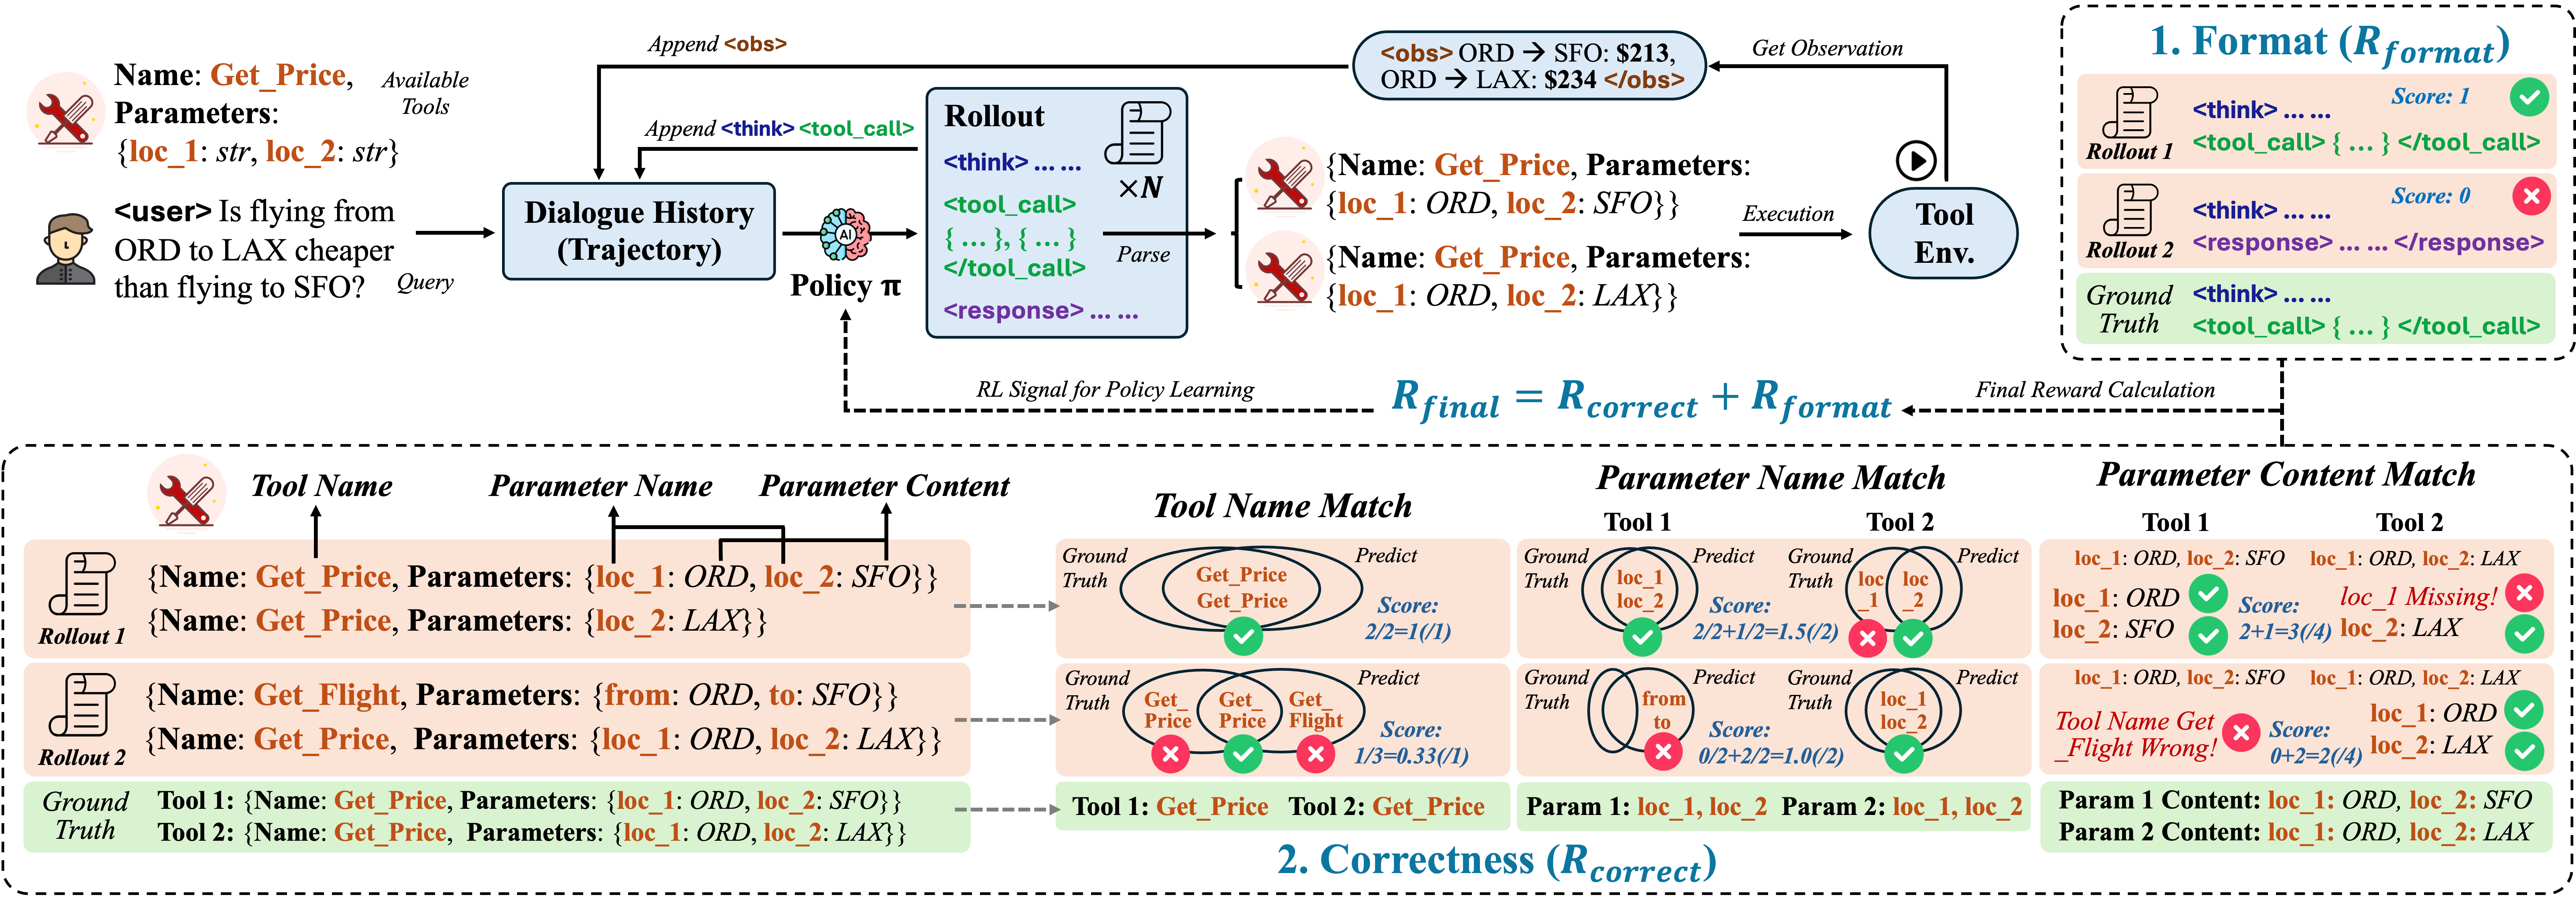
\includegraphics[width=\linewidth]{figures/reward.png}
    \caption{Illustration of TIR rollout and calculation of format and correctness reward.}
    \label{fig:reward}
\end{figure*}

%%%%%%%%%%%%%%%%%%%%%%%%%%%%%%%%%%%%%%%%%%%%

\begin{figure*}[t]
\centering
\resizebox{0.85\textwidth}{!}{
\begin{tcolorbox}[colback=gray!5!white, colframe=blue!75!black, 
title=System Prompt for Training, boxrule=0.3mm, width=\textwidth, arc=3mm, auto outer arc=true]
You are a helpful dialogue assistant capable of leveraging tool calls to solve user tasks and provide structured chat responses.\\
\\
\textbf{Available Tools}\\
In your response, you can use the following tools:\\
\{\{Tool List\}\}\\
\\
\textbf{Steps for Each Turn}\\
1. \textbf{Think:} Recall relevant context and analyze the current user goal.\\
2. \textbf{Decide on Tool Usage:} If a tool is needed, specify the tool and its parameters.\\
3. \textbf{Respond Appropriately:} If a response is needed, generate one while maintaining consistency across user queries.\\
\\
\textbf{Output Format}\\
\textcolor{deepblue}{\textless{}think\textgreater{}} Your thoughts and reasoning \textcolor{deepblue}{\textless{}/think\textgreater{}}\\
\textcolor{deepgreen}{\textless{}tool\_call\textgreater{}}\\
\{``name'': ``Tool name'', ``parameters'': \{``Parameter name'': ``Parameter content'', ``... ...'': ``... ...''\}\}\\
\{``name'': ``... ...'', ``parameters'': \{``... ...'': ``... ...'', ``... ...'': ``... ...''\}\}\\
...\\
\textcolor{deepgreen}{\textless{}/tool\_call\textgreater{}}\\
\textcolor{deeppurple}{\textless{}response\textgreater{}} AI's final response \textcolor{deeppurple}{\textless{}/response\textgreater{}}\\
\\
\textbf{Important Notes}\\
1. You must always include the \textcolor{deepblue}{\textless{}think\textgreater{}} field to outline your reasoning. Provide at least one of \textcolor{deepgreen}{\textless{}tool\_call\textgreater{}} or \textcolor{deeppurple}{\textless{}response\textgreater{}}. Decide whether to use \textcolor{deepgreen}{\textless{}tool\_call\textgreater{}} (possibly multiple times), \textcolor{deeppurple}{\textless{}response\textgreater{}}, or both.\\
2. You can invoke multiple tool calls simultaneously in the \textcolor{deepgreen}{\textless{}tool\_call\textgreater{}} fields. Each tool call should be a JSON object with a ``name'' field and a ``parameters'' field containing a dictionary of parameters. If no parameters are needed, leave the ``parameters'' field an empty dictionary.\\
3. Refer to the previous dialogue records in the history, including the user's queries, previous \textcolor{deepgreen}{\textless{}tool\_call\textgreater{}}, \textcolor{deeppurple}{\textless{}response\textgreater{}}, and any tool feedback noted as \textcolor{brown}{\textless{}obs\textgreater{}} (if exists).\\
\end{tcolorbox}
}
\caption{The system prompt used for TIR's rollout.}
\label{prompt:system}
\end{figure*}

%%%%%%%%%%%%%%%%%%%%%%%%%%%%%%%%%%%%%%%%%%%%

\subsection{TIR Rollout}
\label{sec:tir_rollout}
To enable the model to autonomously generate reasoning traces and tool calls, we utilize a system prompt as shown in \Cref{prompt:system} during rollout. The \textit{Tool List} placeholder denotes the tool set \(\mathcal{T}\), which contains all tools available for invocation. We indicate in the instruction that the LLM should use special tokens \textcolor{deepblue}{\textless{}think\textgreater{}}, \textcolor{deepgreen}{\textless{}tool\_call\textgreater{}}, and \textcolor{deeppurple}{\textless{}response\textgreater{}} to indicates their thoughts, tool calls and responses in output.

As illustrated in \Cref{fig:reward}, when the model output includes \textcolor{deepgreen}{\textless{}tool\_call\textgreater{}}, we automatically parse the tool calls into individual invocations using the model-predicted parameters. The outputs from executions are then inserted into the \textcolor{brown}{\textless{}obs\textgreater{}} field and appended to the dialogue history, whose format is shown in \Cref{prompt:user}, serving as the model's interaction trajectory. Similarly, if the output contains \textcolor{deeppurple}{\textless{}response\textgreater{}}, the corresponding response is parsed and appended to the dialogue history.

It is important to note that \textcolor{deepgreen}{\textless{}tool\_call\textgreater{}} and \textcolor{deeppurple}{\textless{}response\textgreater{}} are not mutually exclusive; they may co-occur within a single output. The user's initial query \( Q \) is placed in the \textit{Initial User Input} placeholder, and any subsequent user inputs are also appended to the dialogue history when present.
% \hongru{maybe also use mathmatical notions?}\cheng{I think figure here could illustrate more clearly. Figure added.}

%%%%%%%%%%%%%%%%%%%%%%%%%%%%%%%%%%%%%%%%%%%%


\subsection{Reward Design}
\label{sec:reward_design}
Rule-based reward mechanisms have demonstrated strong empirical performance and are commonly employed. In our training, we similarly adopt a reward formulation that combines structural and correctness-based components, in line with prior works~\citep{jin2025search, li2025torl, xie2025logic}. Specifically, the format reward assesses whether the model output adheres to the expected structure including thoughts, tool calls, and responses, while the correctness reward evaluates the accuracy of tool invocations. Formally, the overall reward \( R_{\text{final}}(\cdot) \) is decomposed into two components: \( R_{\text{format}} + R_{\text{correct}} \), each described in detail below:

\paragraph{Format Reward.} The format reward \( \mathcal{R}_{\text{format}} \in \{0, 1\} \) checks whether the model output contains all required special tokens in the correct order as specified by the ground truth:

\begin{equation*}
\mathcal{R}_{\text{format}} = 
\begin{cases}
1, & \vcenter{\hbox{\parbox{5.5cm}{if all required fields appear\\and are in the correct order}}} \vspace{8pt}\\
0, & \text{otherwise}
\end{cases}
\end{equation*}

\paragraph{Correctness Reward.} The correctness reward \( \mathcal{R}_{\text{correct}} \in [-3, 3] \) evaluates predicted tool calls \( P = \{P_1, ..., P_m\} \) against ground-truth calls \( G = \{G_1, ..., G_n\} \). It includes three components:

\begin{itemize}[topsep=2pt, leftmargin=10pt, itemsep=0pt]
\item \textit{Tool Name Matching:}
\begin{small}
\begin{equation*}
r_{\text{name}} = \frac{|N_G \cap N_P|}{|N_G \cup N_P|} \in [0, 1]
\end{equation*}
\end{small}
where \( N_G \) and \( N_P \) are the sets of tool names extracted from the ground-truth and predicted tool calls, respectively. 
% \hongru{is this reasonable? suppose Ng = abc, and Np = abd, the reward is 0.5? and if Np=aed, the reward is 0.2? seems have some bias} \cheng{high overlap -> high reward, as we regard those tool calls as parallel calls, why this is biased?} \cheng{N_p should be taken into account to avoid hacking (N_G = abc, N_p = abcdefghi)}

\item \textit{Parameter Name Matching:}
\begin{small}
\begin{equation*}
r_{\text{param}} = \sum_{G_j \in G} \frac{|\text{keys}(P_G) \cap \text{keys}(P_P)|}{|\text{keys}(P_G) \cup \text{keys}(P_P)|} \in [0, |G|]
\end{equation*}
\end{small}
where \( \text{keys}(P_G) \) and \( \text{keys}(P_P) \) represent the parameter names of the predicted and ground-truth tool calls, respectively.

\item \textit{Parameter Content Matching:}
\begin{small}
\begin{equation*}
\begin{split}
r_{\text{value}} = \sum_{G_j \in G} \ \sum_{k \in \text{keys}(G_j)} \mathds{1}[P_G[k] = P_P[k]] \\
\in [0, \sum_{G_j \in G} |\text{keys}(G_j)|]
\end{split}
\end{equation*}
\end{small}
where \( P_G[k]] \) and \( P_P[k] \) represent the values of the parameters for the predicted and ground truth tool calls.

\item Total match score for each match is:
\begin{small}
\begin{equation*}
r_{\text{match}} = r_{\text{name}} + r_{\text{param}} + r_{\text{value}} \in [0, S_{\max}]
\end{equation*}
\end{small}
where \( S_{\max} = 1 + |G| + \sum_{G_j \in G} |\text{keys}(G_j)|\) denotes the maximum possible score.
\end{itemize}

\vspace{5pt} \noindent
The total score is computed by finding the optimal matching between \( P \) and \( G \) to maximize the total match score:
\begin{equation*}
\mathcal{R}_{\text{correct}} = 6 \cdot \frac{R_{\max}}{S_{\max}} - 3 \in [-3, 3]
\end{equation*}
where \( R_{\max} \) denotes the total match score from the optimal matching. The final correctness reward \( \mathcal{R}_{\text{correct}} \) is the normalized reward for the matching process. We empirically set the reward scale within the range of \( [-3, 3] \), with more analysis and ablatiions of reward scale presented in \Cref{sec:analysis}.
% \hongru{a little confused about this equation and sentences, and why need to map to -3 to 3?} \cheng{[-3, 3] is typical correctness (answer) scale (e.g. from LogicRL) to ensure absolute value is larger than format reward. We further conduct ablation analysis in Sec 5 later about value scale.}

The final reward value \( \mathcal{R}_{\text{final}} \) is finally derived as the sum of \( \mathcal{R}_{\text{format}} \) and \( \mathcal{R}_{\text{correct}} \):
\[
\mathcal{R}_{\text{final}} = \mathcal{R}_{\text{format}} + \mathcal{R}_{\text{correct}} \in [-3, 4]
\]

Unlike prior works that often rely on binary or overly simplified reward signals, our design captures the nuanced structure of tool calls by evaluating multiple interdependent components including tool names, parameter schemas, and parameter values. This fine-grained formulation better reflects the complexity of real-world tool use, where correctness cannot be reduced to a single binary criterion. We further validate the impact of this design through comprehensive analysis in \Cref{sec:analysis}.

Overall, our reward design ensures a balanced and interpretable evaluation signal by explicitly separating structural compliance from semantic correctness. By aligning rewards with both format adherence and fine-grained tool call accuracy, the model is guided to produce outputs that are not only syntactically valid but also semantically faithful, which is crucial for downstream tool execution and final task success.
% \hongru{so what is the total reward? combination of corretness and format? need to be clearly explained.}

%%%%%%%%%%%%%%%%%%%%%%%%%%%%%%%%%%%%%%%%%%%%

\subsection{RL Training with GRPO}
\label{sec:rl_training}
To tune the model with structured rewards, we employ GRPO, a variant of PPO that introduces advantage normalization within grouped samples. This normalization helps stabilize training by reducing variance across samples that share a common input context. Let \(\pi_\theta\) represent the current policy.

\paragraph{Normalized Advantage Across Query Groups.}
For each query \( Q \), its responses derived from the rollout form a group \( G_Q \) consisting of multiple responses and their corresponding reward values: 
\[
G_Q = \{ A, (s_1, r_1), (s_2, r_2), \ldots, (s_n, r_n) \}
\]
where \( A \) denotes the ground-truth annotation for \( Q \), and each reward \( r_i \) is computed as the sum of the format and correctness rewards associated with response \( s_i \), i.e., \( r_i = \mathcal{R}_{\text{format}}(s_i, A) + \mathcal{R}_{\text{correct}}(s_i, A) \). For each group, we calculate the mean and standard deviation of the rewards:

\begin{small}
\begin{equation*}
    \mu_Q = \frac{1}{n} \sum_{i=1}^n r_i, \quad 
    \sigma_Q = \sqrt{\frac{1}{n} \sum_{i=1}^n (r_i - \mu_Q)^2}
\end{equation*}
\end{small}

Then, for each sample \( s_i \) in the group, we define the normalized advantage:

\begin{small}
\begin{equation*}
    A_i(s_i | Q) = \frac{r_i - \mu_Q}{\sigma_Q + \eta}
\end{equation*}
\end{small}
where \( \eta \) is a constant to avoid division by zero.

\paragraph{Policy Optimization Objective.}
The policy \( \pi_\theta \) is optimized using the standard clipped PPO objective, adapted with our group-wise normalized advantages:

\begin{small}
\begin{equation*}
\begin{split}
J_{\text{GRPO}}(\theta) = \mathbb{E}_{Q \sim \mathcal{D}} \mathbb{E}_{s_i \sim \pi_\theta} \Big[ 
\min\Big( \frac{\pi_\theta(s_i|Q)}{\pi_{\text{old}}(s_i|Q)} A_i(s_i|Q), \\
\text{clip}\big( \frac{\pi_\theta(s_i|Q)}{\pi_{\text{old}}(s_i|Q)}, 1-\epsilon, 1+\epsilon \big) A_i(s_i|Q) 
\Big) \Big]
\end{split}
\end{equation*}
\end{small}

Unlike the original GRPO formulations, we omit the KL penalty term against a reference model. This design choice encourages the model to more freely adapt its behavior to our custom response format and structured reward signals. In practice, we observe that this leads to faster convergence and comparable performance, while also simplifying the training pipeline.

Overall, this objective guides the policy to generate structurally consistent and semantically accurate tool calls, while group-wise normalization mitigates reward variance across queries, leading to more stable and sample-efficient alignment with task-specific response requirements.

